\chapter{Astroparticle physics and neutrino astronomy}
\label{chap:astro}

The Standard Model (SM) of the particle physics explains almost all available experimental results nowadays. However, it is believed by physicists that it is incomplete, a low energy limit of a more fundamental theory \cite{Maurizio}. It is possible that no accelerator on Earth, in the near or even far future, could reach this high energy limit (above $10^{14}$ GeV). Thus, astroparticle physics may be a key field to understand fundamental physics, since energies above this threshold have already been measured in cosmic radiation. The majority of these cosmic rays come from charged particles that are diverted by large interstellar and intergalactic magnetic fields, randomizing the direction of these particles. In this context, neutrino astronomy plays a fundamental role giving birth to multimessenger astronomy. Almost since their discovery, neutrinos were considered an ideal astronomical messenger \cite{astro_neutrino}. Historically, the astronomy research was centred in the study of incoming photons since the invention of the optical telescope. Photons point back to their source due to the fact that they are electrically neutral, property that is shared with neutrinos. However, photons interact very easily with matter: they are the interaction boson of the electromagnetic force. As a result, objects located behind other structures along the line of sight are harder to detect. Therefore, neutrinos show an advantage with respect to photons: their extremely weak interaction with matter, which is only possible trough the weak force. This allow neutrinos to travel long distances without being deflected or stopped, traversing even whole galaxies. However, these properties also make them quite hard to detect, needing huge experimental apparatus to conduct neutrino astronomy.

In this chapter, we first briefly introduce the history of neutrinos, from their discovery to present time. Then, we explore the possible origin of cosmic neutrinos, their relation with cosmic rays and their theoretical sources. After that, we focus on the physical principles of detection in neutrino telescopes. Finally, we present the history of these telescopes along with some technical details of the currently active detectors, letting the full explanation of ANTARES for other occasion, one of the most important neutrino telescopes, whose collected data is used in this thesis.

\section{Brief history of neutrinos}

Neutrinos were first postulated by Wolfgang Pauli in 1930 \cite{Pauli} in order to explain the continuous electron spectrum in the $\beta$-decay. It was postulated to be an unknown electrically neutral particle with spin 1/2 due to the conservation of quantum numbers. The word \textit{neutrino} was coined by Enrico Fermi, who used it during a lecture in Paris in 1933 \cite{FermiNeutrino}. The first theoretical estimation of the cross section of a neutrino interacting with a nucleus to produce an electron and a proton was obtained by H. Bethe and R. Peierls soon after the Fermi theory was proposed \cite{bethe}. Their calculations were very similar to today's and concluded that there was probably no practical way of ever detecting neutrinos. The first physicist who challenged this opinion was B. Pontecorvo in 1946 \cite{pontecorvo}. He proposed the Cl-Ar radiochemical method of neutrino detection which is based on the reaction

\begin{equation}
	\nu_e + ^{37}\mathrm{Cl} \rightarrow e^- + ^{37}\mathrm{Ar}.
\end{equation}

Even though this method was not the basis for the first neutrino detection, it allowed many years later the observation of solar neutrinos in the first solar neutrino experiment \cite{solarneutrinos}. In 1956, Clyde L. Cowan and Frederick Reines \cite{Clyde} confirmed the first detection of neutrinos (actually, anti-neutrinos) coming from the Savannah River nuclear power plant through the inverse $\beta$-decay. They used a liquid scintillator loaded with CdCl$_2$ as the target for the anti-neutrinos produced in the nuclear reactor. Since then, many other discoveries have followed. In 1962 the famous Brookhaven experiment discovered the existence of a second family of lepton: muons and their respective neutrinos. More big discoveries include the first measurement of the solar neutrino flux at the Homestake experiment \cite{solar} and the detection of extragalactic neutrinos from the supernova SN1987A by Super-Kamiokande \cite{galactic1}.

Nowadays, neutrinos are part of the Standard Model of Particles and they are well understood by theoretical and experimental physics, even though open questions remain. They come in three different flavours \cite{neutrino_muon, neutrino_tau} as their left handed component forms a weak isospin doublet with the corresponding left handed component of the massive charged leptons: $e$, $\mu$ and $\tau$. According to the Standard Model, neutrinos are supposed to be massless, hence neutrinos only interaction is through the weak force. However, in 1998 the Super-Kamiokande experiment announced evidence that the observation of atmospheric neutrinos could only be explained by assuming a transformation between neutrino flavours \cite{Super}. This phenomenon is called Neutrino Oscillation and it is currently explained assuming that neutrinos do have a mass. If neutrinos are massive, the eigenstates of the weak interaction may not correspond to those of free propagation ($\nu_1$, $\nu_2$, $\nu_3$). Thus, after the creation of any neutrino lepton flavour ($\nu_l$) it becomes a quantum superposition of the propagation states, where the mass of the neutrino is definite, through the so-called PMNS or lepton mixing matrix \cite{PMNS2, PMNS}:

\begin{equation}
	|\nu_i\rangle = \sum_{l} U_{li}^{\mathrm{PMNS}} \, |\nu_l\rangle
\end{equation}

This fact posits one of the biggest inconsistencies in modern physics and opens the door to the understanding of a more fundamental particle physics theory.

\section{The origin of cosmic neutrinos}

The origin of cosmic neutrinos is theoretically linked with the origin of cosmic rays (CRs), existing several mechanisms that postulate this connection. Thus, the sources of both types of radiation are expected to be the same in many cases. In this way, we first briefly present here the cosmic rays and, then, their connection to cosmic neutrinos.% We also enumerate their potential sources.

\subsection{Cosmic rays}

In the decade of 1910, Viktor F. Hess \cite{Hess1912} found the first evidences of cosmic radiation. This radiation was mainly composed of high energy charged particles (what we call CRs nowadays) and ionizing photons (X-rays and $\gamma$-rays). The majority of high-energy particles in CRs is composed of protons and, secondarily, by $\alpha$ particles. How and where CRs are produced remains a mystery \cite{Agus}, due to the fact that they are deflected in their path to the Earth by the large electromagnetic fields that many astrophysical objects produce. For the ionizing photons, things are somewhat clearer. Since they point back to their source, known optical astrophysical counterparts can often be identified. Their energy spectra are satisfactorily explained by electron acceleration followed by synchrotron radiation and inverse Compton scattering.% There are some clues that both CRs and the ionizing ration must be produced by the same astrophysical objects.

The CR flux above GeV can be described by a piecewise power-law function \cite{energy_spec}:

\begin{equation}
\frac{\mathrm{d}\phi}{\mathrm{d}E} \propto E^{-\gamma},
\end{equation}

where $E$ is the energy of the primary particle and $\gamma$ is the so-called spectral index. This index changes in a few points of the spectra called \textit{knees} and the flux is fully suppressed at $\sim 100$ EeV. This can be seen in \autoref{fig:CR}. The spectral index is about $2.7$ from several GeV to $\sim$400 TeV, where it changes to $3.3$ in the knee. The spectrum \textit{breaks} after that point in what is called the \textit{second knee} at $\sim$500 PeV. Then, it stays mostly constant until an energy of $\sim$3 EeV, where the index changes again to $2.6$ in a flattening called the \textit{ankle}. The decrease in the CR flux at $\sim$60 EeV possibly corresponds to the predicted Greisen-Zatsepin-Kuzmin (GZK) cutoff \cite{GZK}. It is due to the fact that CRs above this energy have a high probability to interact with the Cosmic Microwave Background (CMB) mainly through the Delta resonance (see \autoref{sec:CR-gamma}), producing pions.

%FROM AGUSTIN THESIS
%It continues almost constant until an energy of $\sim$3 EeV, where it changes again to 2.6 in a flattening called the \textit{ankle}. At $\sim$500 PeV there is evidence of the existence of a break in the spectrum called the “second knee”. CRs above the ankle are usually called Ultra High Energy CRs (UHECRs) and the flux is suppressed above 100 EeV. This decrease in the CR flux possibly corresponds to the predicted Greisen-Zatsepin-Kuzmin (GZK) cutoff [8, 9], and is due to the fact that CRs above 60 EeV have a high probability to interact with the Cosmic Microwave Background Radiation (CMBR) through the Delta resonance (see section 1.3), producing pions. 

\begin{figure}[htbp]
	\centering
	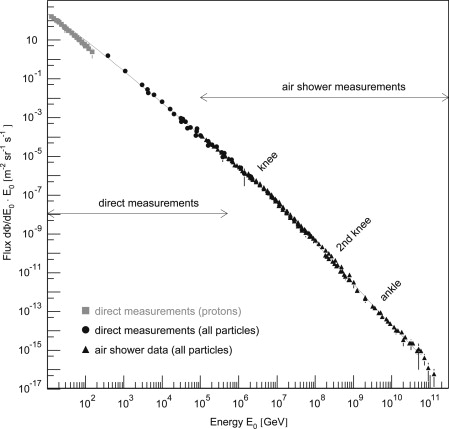
\includegraphics[width=.55\textwidth]{figs1/CRspectrum}
	\caption{\label{fig:CR}All-particle energy spectrum of CRs as measured directly with detectors above the atmosphere and with air shower detectors. Figure taken from \cite{energy_spec}.}
\end{figure}

The features of the CR spectrum are probably indications of the different source populations in energy range and location. Below the knee, sources are believed to be of galactic origin. Above the ankle, the decrease is possibly due to the CR sources reaching their maximum possible energy or to the fact that CRs are able to escape from the galactic magnetic field. In contrast, CRs above the ankle are believed to correspond to populations of extragalactic sources, since the astrophysical objects in the galaxy do not meet the necessary requirements to accelerate them at such energies.

\subsection{CR--$\boldsymbol{\gamma}$--$\boldsymbol{\nu}$ relation}
\label{sec:CR-gamma}

%As mentioned, there are clues that CRs and $\gamma$-radiation are produced by the same astrophysical sources. The connection between these two kinds of radiation and the production of

The connection between CRs and $\gamma$-radiation with the production of cosmic neutrinos is basically due to the interactions of CRs with the environment where they are produced. Since CRs are mainly accelerated protons, their interactions can be reduced to two types:

\begin{enumerate}[label=\textbullet]
	
    \item $\boldsymbol{p\,\gamma}$ \textbf{processes}. The most significant one is the Delta resonance:
	
	$$
	p\,\gamma \rightarrow \Delta^+ \left\{\begin{aligned}
	& \xrightarrow{\text{2/3}} p\,\pi^0 \\
	& \xrightarrow{\text{1/3}} n\,\pi^+ 
	\end{aligned}\right.
	$$
	
	This process is particularly interesting in the case of the interaction of CRs with the CMB, the GZK effect, which is expected to significantly reduce the CR flux above $\sim$100 EeV and produce diffuse fluxes of $\gamma$-rays and neutrinos. Thus, a neutrino detected with an energy above that cutoff limit has certainly a cosmic origin, since it cannot be produced by CRs in the atmosphere, which is the major background contribution in the detectors (see \autoref{subsec:background}).
	
	\item $\boldsymbol{p\,p}$ \textbf{processes}. If the matter density of the environment is larger than that of the radiation, CR interactions are dominated by $p\,p$ processes,  the most frequent being:
	
	$$
	\begin{aligned}
	p\,p \rightarrow p\,p\,\pi^0 \quad &\quad p\,p \rightarrow p\,n\,\pi^+ \\
	p\,n \rightarrow p\,n\,\pi^0 \quad &\quad p\,n \rightarrow p\,p\,\pi^-
	\end{aligned}
	$$
\end{enumerate}

These are hadronic processes, but they can produce leptons through pions that frequently decay into photons and leptons:

$$
\setlength{\jot}{2pt}
\begin{aligned}
\pi^0 \rightarrow & \,\gamma\,\gamma \\[15pt] % <— extra vertical space here
\pi^+ \rightarrow & \,\mu^+ \, \nu_\mu \\
& \hookrightarrow e^+ \, \nu_e \, \bar{\nu}_\mu
\end{aligned}
\qquad\qquad
\begin{aligned}
\pi^- \rightarrow & \,\mu^- \, \bar{\nu}_\mu \\
& \hookrightarrow e^- \, \bar{\nu}_e \, \nu_\mu
\end{aligned}
$$

Thus, the decay of pions from CRs are related to $\gamma$-ray and neutrino production. The ratio $\gamma/\nu$ depends on the rate of $p\,p$ and $p\,\gamma$ processes. Therefore, astrophysical studies based on photons and neutrinos are complementary and necessary to understand the underlying physics of astronomical objects.

\section{Cosmic neutrino sources}

Cosmic neutrinos can be produced in a wide variety of astrophysical objects and through several mechanisms and exotic processes \cite{Agus, sources, sources2, sources3}. The sources can be divided in two categories: galactic and extragalactic sources.

\subsection{Galactic}

\begin{enumerate}[label=\textbullet]

	\item Shell-type Supernova Remnants (SNRs): In a supernova most of the star material is ejected at velocities up to $10\%$ the speed of light. The shock waves generated against the interstellar medium creates the proper conditions to induce particle acceleration. Interaction of these CRs with previously expelled star material and interstellar medium would give rise to neutrino and gamma-ray fluxes.
	
	\item Pulsar Wind Nebulae (PWNe) or pleirons: It refers to a particular kind of SNRs where the supernova left a neutron star or pulsar as remnant. This compact object, with a strong magnetic field and a fast rotation, induces a continuous particle acceleration that flows out in jets.
	
	\item X-Ray Binaries (XRBs): Binary star systems where one of the components is a collapsed object such as a white dwarf, a neutron star or a black hole. The companion star fuels material into the compact partner forming an accretion disk around it. On this accretion process, falling material reach temperatures high enough to emit X-rays.
	
	\item Galactic centre: The centre of the Milky Way hosts a supermassive black hole (Sagittarius A*) surrounded by multiple SNRs, PWNe and XRBs as well as other TeV $\gamma$-ray sources. Neutrino emission seems likely since meson decay is the only feasible mechanism able to diffuse $\gamma$-ray emission in this region.
	
\end{enumerate}

\subsection{Extragalactic}

\begin{enumerate}[label=\textbullet]

	\item Gamma-Ray Bursts (GRBs): Short-lived flashes with the highest known peak luminosities, being the the most energetic events ever detected. They are linked with asymmetric supernovas whose jets point towards the Earth and with compact objects merging. As transitional short events, their time information allows to put strong constrains on predictions.
    
	\item Active Galactic Nuclei (AGNs): In terms of time-integrated energy output and sustained luminosity, their energy release far exceeds that of any other known population, such as SNRs or GRBs. Roughly 1\% of all bright galaxies possess an active nucleus in which the equivalent of the radiation power of more than the combination of all stars in our galaxy is radiated from a region smaller than the size of the solar system. The brightest AGNs on $\gamma$-ray emission are called \textit{blazars}. These objects are expected to be AGNs with active relativistic jets pointing towards the Earth. The object PKS 0735+17 is a particular case of these objects, which will be the first use case for the method developed in \autoref{chap:ml}. 
	
	\item Starburst galaxies: These galaxies host regions with a very high star formation rate compared to regular galaxies. As a consequence, supernovas take place frequently enough to expect an important CR production.
	
	\item Galaxy clusters: They are the largest gravitationally bounded objects in the universe. Their possible neutrino production is expected from $p\,p$ interactions between CRs and intracluster material.
	
	\item Cosmogenic (GZK) neutrinos: A diffuse neutrino flux is expected to be produced as a consequence of the GZK effect through the Delta resonance when CRs have enough energy.
\end{enumerate}

\section{Detection principle}

The properties that make neutrinos good candidates as astronomical messengers also make them very hard to detect. The first proposal to detect cosmic neutrinos was described by M. A. Markov in 1960 \cite{astro_neutrino}. In order to discriminate the incoming direction, neutrinos have to be detected indirectly through their interactions with matter at the Earth. The proposal was to detect charged secondary particles from the neutrino-nucleon interaction, such as muons, via emission of Cherenkov light \cite{Cheren}. The detector, a three-dimensional array of photomultiplier tubes (PMTs) inside a transparent medium like water or ice, collects the Cherenkov radiation induced by the passage of the relativistic charged particles inside or near the instrumented volume. Due to the low cross section of the neutrino-nucleon interaction, the volume of detection is needed to be very large --at the order of 1000 m$^3$--, so it was proposed to set the detectors deep in the ocean or in an underground lake. The information registered by the PMTs is used to infer the arrival direction of the parent neutrino and an estimation of its energy. Thus, the basic idea of a neutrino telescope was born.

A problem with this detection mechanism is that charged particles produced by other mechanisms are also detected. Huge amounts of muons are produced by CRs colliding with the atmosphere. Therefore, neutrino telescopes are optimised to detect the light from up-going particles produced by neutrinos which have traversed the Earth. Hence, the detection of down-going atmospheric muons, which is the major background contribution, is heavily reduced. Nevertheless, contributions to the background events occur due to the production of atmospheric neutrinos and bioluminescence. These topics are discussed in detail in the following sections.

\subsection{Neutrino interactions with matter}

Neutrinos only interact through the weak force. There exists two possible channels of interaction with matter (typically with a nucleus, $N$) \cite{neutrino_interactions}: 

\begin{enumerate}[label=\textbullet]
	\item Charged Current (CC): The interaction is produced through the $W^{\pm}$ boson.
    
	$$
    \nu_l \, N  \rightarrow  \,l^- +\mathrm{hadronic~jet} \qquad \qquad \bar{\nu}_l \, N  \rightarrow  \,l^+ +\mathrm{hadronic~jet}
    $$
    
    \hide{
    $$
    \setlength{\jot}{2pt}
	\begin{aligned}
	\nu_l \, N  \rightarrow & \,l^- +\mathrm{hadronic~jet} \\
	\bar{\nu}_l \, N  \rightarrow & \,l^+ +\mathrm{hadronic~jet}
	\end{aligned}
	$$
    }
	
	\item Neutral Current (NC): The interaction is produced through the $Z^0$ boson.
	
    $$
	\nu \, N  \rightarrow \nu \, N
	$$
	
\end{enumerate}

Depending on the type of interaction and the lepton flavour, two types of event signatures can be detected in a neutrino telescope \cite{inter}. Track-like events are originated from CC of muon-(anti)neutrino interactions ($\nu_\mu^{CC}$). The muon produced can travel very long distances before decaying. Thus, this kind of events are well suited for direction reconstructions. The angular difference between the primary neutrino and the muon is usually $<1^\circ$ for neutrino energies around 1 TeV, with finer alignments as the energy increases.

The second type of signatures are cascades, also known as shower-like events. These are produced by all NC interactions and by electronic CC ($\nu_l^{NC}$, $\nu_e^{CC}$). In the NC interactions, the energy transferred to the nucleus produce a hadronic shower, while a residual part of the energy is carried by a secondary neutrino. In the electronic CC, the produced electron rapidly loses energy via \textit{bremsstrahlung} and pair production, generating an electromagnetic shower and depositing almost all the energy near the interaction vertex. Since cascades do not spread much, direction reconstruction of shower events is typically more difficult than that of track events, whereas for the energy reconstruction, the trend is the opposite.

The $\nu_\tau^{CC}$ interactions are usually treated separately, since they can produce both shower and track events, depending on the energy of primary neutrinos and the nature of the secondary interaction. In contrast to muons, tauons have a much shorter lifetime, so they travel only from metres to kilometres, depending of their energy, before decaying. If the tauon decays into a muon, the resulting particle can produce a long track, being indistinguishable from a $\nu_\mu^{CC}$ interaction by the detector. If the tauon produces an electron or a tau-neutrino, the result is an electromagnetic or hadronic shower, respectively, generating a ``double bang'' signature, which refers to the sequence of two consecutive cascades. \autoref{fig:inter} shows schematic views of the most relevant processes.

\begin{figure}[htbp]
	\centering
	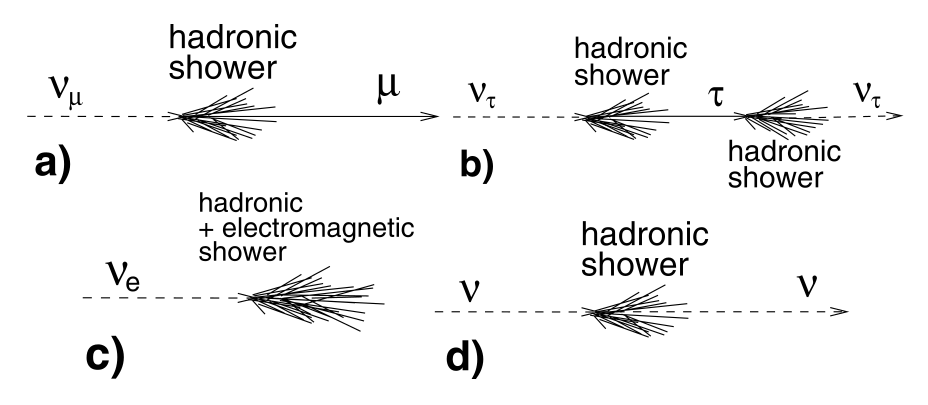
\includegraphics[width=.6\textwidth]{figs1/CC_NC}
	\caption{\label{fig:inter}Schematic view of the most relevant event signatures in a neutrino telescope: $\nu_\mu^{CC}$ (a), $\nu_\tau^{CC}$ double bang (b), $\nu_e^{CC}$ (c) and all flavour $\nu^{NC}$ (d). Figure taken from \cite{image_inter}.}
\end{figure}


\subsection{Cherenkov radiation}

Cherenkov radiation is emitted by charged particles crossing a dielectric medium with speed exceeding that of light in the medium \cite{Cheren}. The charged particle polarizes the molecules along its trajectory, but only an overall dipole moment is present when the particle moves faster than light in the medium. Cherenkov light is emitted when the electrons of the dielectric medium restore themselves to equilibrium after the disruption has passed, creating a coherent radiation emitted in a cone with a characteristic angle $\theta_C$:

\begin{equation}
\cos(\theta_C)  = \frac{1}{\beta \, n},
\end{equation}

where $\beta = v/c$ is the particle velocity in units of $c$ and $n$ is the medium refractive index. 

The emission spectrum is continuum and its intensity increases with the frequency up to blue and ultraviolet (UV) wavelengths, above which, the emission is no longer possible. The amount of Cherenkov photons ($N_\gamma$) emitted by a particle of charge Z per unit wavelength interval (d$\lambda$) and unit distance traveled (d$x$) is \cite{N_cheren}:

\begin{equation}
\frac{\mathrm{d}N_\gamma}{\mathrm{d}\lambda \mathrm{d}x} = \frac{2\pi\alpha Z^2}{\lambda^2}\left( 1-\cos^2(\theta_C) \right),
\end{equation}

where $\alpha$ is the fine structure constant.

\subsection{Background noise} % contamination? events?
\label{subsec:background}

There are challenges using Cherenkov light of secondary particles as detection principle. First, other processes in the atmosphere produce charged particles that are detected by neutrino telescopes. CR showers in the atmosphere produce a continuous isotropic flux of neutrinos. They are called atmospheric neutrinos and are the biggest source of noise when trying to detect cosmic neutrinos. Except for ultra-high energy events, this contribution to the background noise impedes event to event detection. Detections are then based on statistical analysis.

Second, CR showers in the atmosphere produce atmospheric muons. Since the telescopes only detect charged particles, they leave the same signature as a secondary particle from a neutrino interaction. To diminish the amount of atmospheric muons being detected as neutrino muons, neutrino telescopes usually point downwards, using the Earth as a shield. This is because the probability of a muon traversing the Earth is null. However, upward reconstruction from a downwards particle, although unlikely, can happen.

Therefore, a good understanding and estimation of the background is capital in neutrino telescopes. It is needed to find evidences of a cosmic neutrino flux from event excesses, differences in spectrum energy or in arrival directions.% \nota{Tal vez ampliar un poco, ya veremos}


\section{Neutrino telescopes}

The first attempt of building a neutrino telescope was the DUMAND project \cite{Dumand} in the late 1970s. It aimed to deploy a detector in the Pacific Ocean, near to the island of Hawaii. The project was cancelled due to technical and financial problems, but it set the basis for the following neutrino telescopes. The relay of the high-energy neutrino astronomy was taken by the Baikal telescope \cite{Baikal1}, located in the depths of the Russian Lake Baikal, and by the AMANDA telescope \cite{Amanda}, under the ice of the South Pole. The experience of the DUMAND project was taken up by ANTARES \cite{Antares}, leading afterwards to the, already under construction, largest deep-sea neutrino telescope, KM3NeT \cite{km3net}. The Italian NEMO \cite{NEMO} and the Greek NESTOR \cite{NESTOR} initiatives, although never completed, also contributed to the development that eventually converged in KM3NeT. In parallel, there is also a new project, called P-ONE, still in the research and development stage \cite{Pone}, and initiatives in China in the same direction, such as TRIDENT \cite{TRIDENT}. Here, we briefly detail the three currently active detectors.

%The first attempt of building a neutrino telescope was the DUMAND project \cite{Dumand} in the late 1970s. It aimed to deploy a detector in the Pacific ocean, near to the island of Hawaii. The project was cancelled due to technical and financial problems, but it set the basis for the following neutrino telescopes. The relay of the high-energy neutrino astronomy was taken by the Baikal telescope \cite{Baikal1}, located in the depths of the Russian Lake Baikal, and by the AMANDA telescope \cite{Amanda}, under the ice of the South Pole. The experience of the DUMAND project was taken up by ANTARES\cite{Antares}, leading afterwards to the, already under construction, largest deep-sea neutrino telescope, KM3NeT \cite{km3net}. There is also a new project, called P-ONE, still in the research and development stage \cite{Pone}. The ANTARES telescope will be detailed in \autoref{chap:antares}. In the following paragraphs, the three currently active detectors will be briefly detailed.

\subsubsection*{Baikal-GVD}

The Baikal neutrino detector, first deployed in 1993, underwent a significant upgrade to become the Baikal Gigaton Volume Detector (Baikal-GVD) \cite{Baikal}. Since its inception, the sensitivity and coverage of the experiment have progressively improved. Currently, the facility incorporates 2304 MPTs deployed at depths reaching up to 1366 meters. The detector’s infrastructure consists of vertical strings anchored to the lakebed and stabilized by buoyant systems at their upper ends. Each string has 36 optical modules (OMs), with every module equipped with a 10-inch, high-quantum-efficiency PMT oriented downward to optimize detection capabilities.

\subsubsection*{IceCube}

The IceCube Neutrino Observatory, constructed between 2005 and 2010, is the successor to the AMANDA (Antarctic Muon and Neutrino Detector Array) experiment located in the South Pole’s glacial ice \cite{IceCube}. Its detector encompasses a cubic kilometre of pristine Antarctic ice, optimized for high transparency. The infrastructure comprises 86 vertical strings positioned above the bedrock at depths of 1.5 to 2.5 kilometres. These strings, spaced 125 meters apart in a grid of equilateral triangles, hold 5,160 Digital Optical Modules (DOMs). Each DOM features a spherical, pressure-resistant housing containing a 25-centimetre PMT and digitization electronics. Modules are spaced 17 meters vertically along each string. To improve sensitivity to low-energy neutrinos, a dense central sub-array named DeepCore employs high-quantum-efficiency PMTs. The observatory also integrates IceTop, a surface-level cosmic ray detector, forming a comprehensive detection system. Full operational data collection began in May 2011. In 2014, IceCube achieved a milestone by confirming the first astrophysical neutrinos of cosmic origin \cite{ice}. Since then, IceCube has measured a diffuse flux of high-energy astrophysical neutrinos and provided important constraints on their energy spectrum. The collaboration has also reported high-profile detections of neutrinos coincident with blazar flares, contributing to the identification of potential cosmic neutrino sources \cite{iceblazar, icediffuse}.


\subsubsection*{KM3NeT}

The Cubic Kilometre Neutrino Telescope (KM3NeT) is still under construction, but already taking data since 2019. It is a deep-sea neutrino telescope in the Mediterranean Sea and, once completed, it will be the largest neutrino telescope in the world. It is composed of two separate detectors: ARCA and ORCA (Astroparticle/Oscillation Research with Cosmics in the Abyss) \cite{km3net1}.

ARCA’s primary scientific objective is to identify high-energy neutrinos originating from cosmic sources. Specifically, the experiment focuses on investigating potential cosmic ray accelerators within the Milky Way to detect neutrino emissions associated with these astrophysical phenomena. Located approximately 100 kilometres off-shore Portopalo di Capo Passero (Italy), the infrastructure operates at a depth of about 3,500 metres. The finalized design includes two independent blocks, each composed of 115 Detection Units (DUs), collectively instrumenting a volume of roughly one cubic kilometre. Each DU extends vertically for approximately 700 meters, with 18 DOMs distributed at 36-meter intervals starting 80 meters above the seabed. The horizontal separation between adjacent detection strings is approximately 95 metres. At the time of writing this thesis (October~2025), it is composed of 51 DUs. Remarkably, ARCA was able to detect in February 2023 --when only 21 DUs were working-- a neutrino with the highest energy ever recorded \cite{nature}.

ORCA is optimized for less energetic neutrinos, in the range of a few hundreds GeV, in order to study oscillations and mass ordering, among other exotic physics. Located about 40 kilometres off-shore Toulon (France), at a depth of 2,450 metres. When complete, it will be composed of only one building block with 115 DUs, each DU holding 18 DOMs spaced 9 metres apart in the vertical direction. The horizontal spacing between each DU string will be of around 20 metres. ORCA has then a smaller, but more densely instrumented volume compared to ARCA, better aligned to focus in a lower energy range. At the time of writing this thesis (October~2025), ORCA is composed of 24 DUs.

